\chapter{Field Programmable Gate Arrays}\label{cap_fpga}

{
    \textit{Field Programmable Gate Arrays}---ou \textit{FPGAs}---são circuitos
    integrados que permitem o desenvolvimento de circuitos lógicos
    reconfiguráveis. Por serem reprogramáveis, as \textit{FPGAs} geram uma
    grande economia em tempo de desenvolvimento e em custos como os de
    prototipagem, validação e manufatura do projeto em relação aos circuitos de
    aplicações específicas, os \textit{ASICs}. As \textit{FPGAs} podem ser
    tanto o passo intermediário no projeto de um \textit{ASIC} quanto o meio
    final do projeto quando a reconfigurabilidade e os preços muito mais
    acessíveis forem fatores importantes.
}

{
    Cada fabricante de \textit{FPGAs} possui seus \textit{softwares} de
    desenvolvimento, ou \textit{SDKs}. A indústria de \textit{hardware} é
    extremamente protecionista com sua propriedade intelectual, sendo a maioria
    dessas ferramentas de código proprietário. Para a Intel Altera®, essa
    plataforma é o Quartus Prime®.
}

{
    \textit{FPGAs} mais modernas possuem, além do arranjo de portas lógicas,
    blocos de memória, \textit{PLLs}, \textit{DSPs} e \textit{SoCs}. Os blocos
    de memória internos funcionam como a memória \textit{cache} de um
    microprocessador, armazenando os dados próximo ao seu local de
    processamento para diminuir a latência. Os \textit{PLLs} permitem criar
    sinais de \textit{clock} com diversas frequências a partir de um relógio de
    referência, e podem ser reconfigurados a tempo de execução. \textit{DSPs}
    são responsáveis pelo processamento de sinais analógicos discretizados, e
    podem ser utilizados como multiplicadores de baixa latência. Já os
    \textit{SoCs} são microprocessadores como os ARM® presentes
    em celulares, e são capazes de executar sistemas operacionais como o Linux.
}

{
    Além de disponíveis na forma de \textit{chips} para a integração com placas
    de circuito impresso customizadas, as \textit{FPGAs} possuem \textit{kits}
    de desenvolvimento com diversos periféricos para auxiliar no processo de
    criação de soluções. Esses \textit{kits} são a principal ferramenta de
    aprendizagem no universo dos circuitos reconfiguráveis. No Laboratório de
    Informática da UnB, as placas \textit{terasIC DE1-SoC} com a \textit{FPGA
    Intel® Cyclone V SoC} estão disponíveis para os alunos de OAC desenvolverem
    seus projetos.
}

\clearpage

\section{Arquitetura Generalizada de uma FPGA}
{
    De forma genérica, uma \textit{FPGA} possui blocos lógicos, chaves de
    interconexão, blocos de conexão direta e portas de entrada e saída,
    conforme apresentado na Figura~\ref{fig:fpga_general_arch}.
}

\begin{figure}[H]
\centering
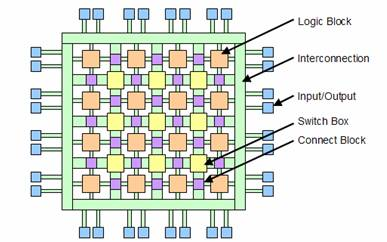
\includegraphics[width=.7\linewidth]
    {../images/fpga_architecture_abstraction_-_olin_college.jpg}
    \caption[Abstração da arquitetura de uma FPGA]
        {Abstração da arquitetura de uma FPGA \quad Fonte: Olin College of
            Engineering}\label{fig:fpga_general_arch}
\end{figure}

{
    Os blocos lógicos possuem \textit{lookup tables}, registradores, somadores
    e multiplexadores. É neles que a lógica reconfigurável é implementada.
}

{
    Já as chaves de interconexão são responsáveis por conectar os diversos
    blocos da \textit{FPGA}. A Figura~\ref{fig:fpga_switch_box} exemplifica
    como é feito o roteamento da malha de interconexão. Os blocos de conexão
    direta são um tipo especial de chave de interconexão, e sua função é ligar
    blocos lógicos adjacentes.
}

{
    Por fim, as portas de entrada e saída conectam a \textit{FPGA} ao ``mundo
    externo'' e.g. \textit{drivers} de áudio e vídeo.
}

\begin{figure}[H]
\centering
\includesvg[width=.5\linewidth]
    {../images/switch_box_wikimedia.svg}
    \caption[Funcionamento da chave de interconexão]
        {Funcionamento da chave de interconexão \quad Fonte: Wikimedia
        }\label{fig:fpga_switch_box}
\end{figure}

\clearpage


\section{Arquitetura da FPGA Cyclone V SoC}
{
    A Figura~\ref{fig:cyclone_v_arch} apresenta a arquitetura da \textit{FPGA
    Cyclone V SoC}.
}

\begin{figure}[H]
\centering
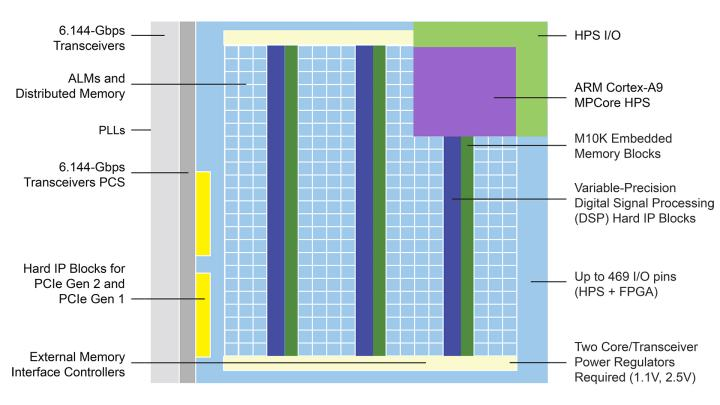
\includegraphics[width=1\linewidth]
    {../images/altera_cyclone_v_soc_architectural_downscale.jpg}
    \caption[Arquitetura da FPGA Intel Cyclone V SoC]
        {Arquitetura da \textit{FPGA Altera Cyclone V SoC} \quad Fonte: Intel
        }\label{fig:cyclone_v_arch}
\end{figure}

    \subsection{Adaptative Logic Modules}
    {}

    \begin{figure}[H]
    \centering
    \includesvg[inkscapeformat=png,width=1\linewidth]
        {../images/intel_alm_high_level.svg}
        \caption[Diagrama de blocos de um ALM]
            {Diagrama de blocos de um ALM\quad Fonte: Intel
            }\label{fig:fpga_alm}
    \end{figure}


    \subsection{Embedded Memory Blocks}
    {}

    \subsection{Hard Processor System}
    {}

    \subsection{Phase-Locked Loops}
    {}

\section{A Placa de Desenvolvimento DE1-SoC}


